\section{考察}
結果として,フラフープに対して左右1mまでであれば自分の位置を補正しながらフラフープを通り抜けるシステムを構築する事が出来た.
しかし

\begin{figure}[htbp]
  \begin{center}
    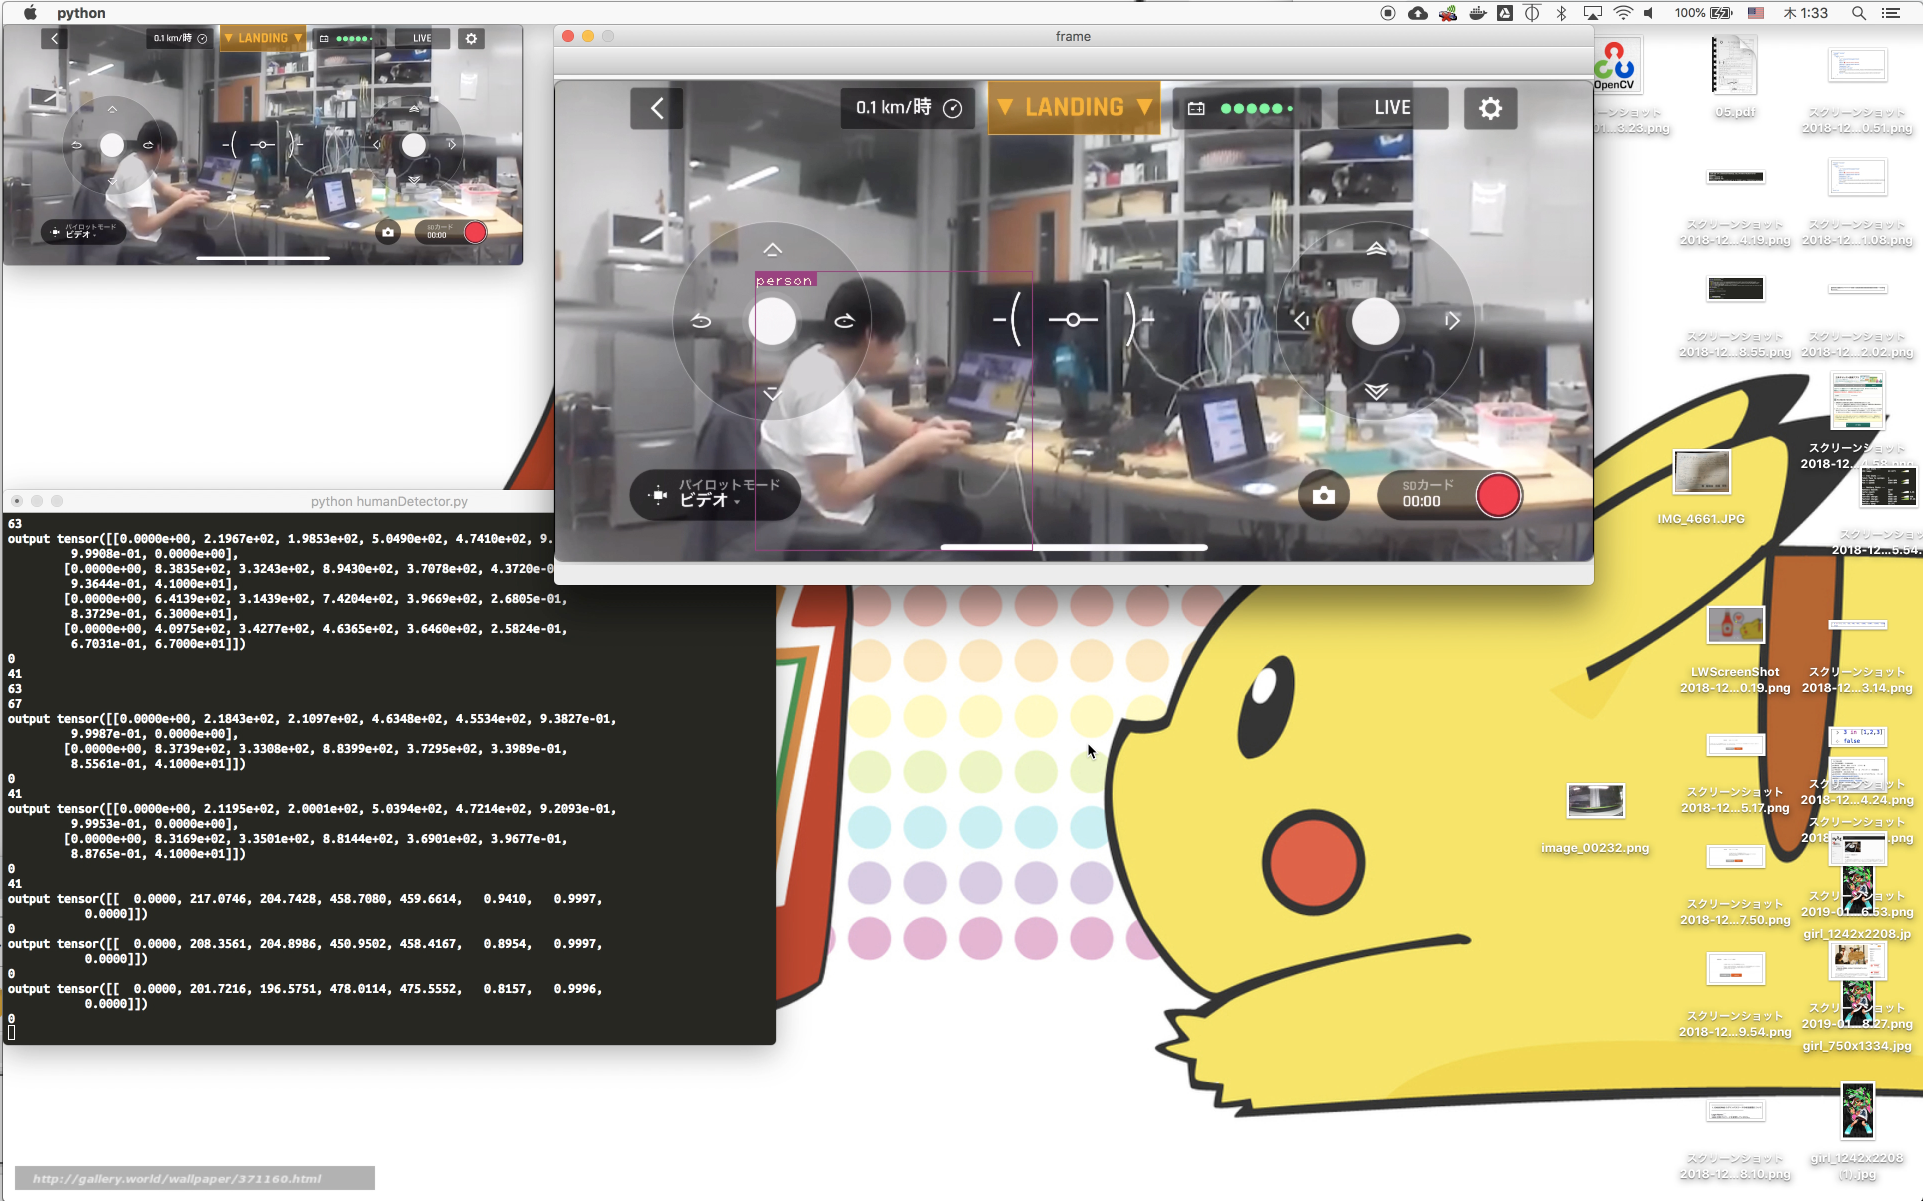
\includegraphics[clip,width=7.0cm]{img/sys-image.png}
    \caption{PC上の表示(上が配信映像,下が検出時の映像)}
    \label{fig:sys}
  \end{center}
\end{figure}

今後はドローンレースの自動化に向けて今回の飛行モデルをベースに検出モデル,制御ルールをアップデートしていく形で実装を進めて行きたい.
